
\documentclass[
	12pt,				% tamanho da fonte
	oneside,			% para impressão apenas no verso. Oposto a twoside
	a4paper,			% tamanho do papel.
	]{article}
% ---
% Pacotes
% ---
\usepackage{cmap}				% Mapear caracteres especiais no PDF 
\usepackage{times}			% Usa a fonte Latin Modern
\usepackage[T1]{fontenc}		% Selecao de codigos de fonte.
\usepackage[utf8]{inputenc}		% Codificacao do documento (conversão automática dos acentos)
\usepackage[USenglish]{babel}
\usepackage{indentfirst}		% Indenta o primeiro parágrafo de cada seção.
\usepackage{nomencl} 			% Lista de simbolos
\usepackage{color}				% Controle das cores
\usepackage{color, colortbl}
\usepackage{graphicx}			% Inclusão de gráficos
\usepackage{tabularx}           % in the preamble
\usepackage{amsmath,amssymb}
\usepackage{multirow}
\usepackage{lscape}
\usepackage{caption,booktabs,array}
\newcommand{\rowgroup}[1]{\hspace{-1em}#1}
\usepackage[flushleft]{threeparttable}
\usepackage{subfigure}
\usepackage{rotating}
\usepackage{pdflscape}
\usepackage{comment}
\usepackage{setspace}
\usepackage{geometry}
\usepackage{multicol}
\usepackage{siunitx}
\usepackage{float}
\usepackage{blindtext}
\usepackage{chngcntr} %Para recomecar do 1 a numeracao das tabelas dos anexos
\usepackage{breqn} 
\hyphenpenalty=10000
\makeatletter% Set distance from top of page to first float
\setlength{\@fptop}{5pt}
\makeatother
\usepackage{hyperref}
	
\definecolor{Gray}{gray}{0.9}
% 
% Estout related commands
% 
\renewcommand{\arraystretch}{1.1}
\newcommand{\sym}[1]{\rlap{#1}}
% \tablefragment: input a Stata-generated table fragment inside a tabular.
% The LaTeX \input opens a group and breaks at the start of an alignment row;
% the TeX primitive \@@input is expansion-safe inside tabulars.
\makeatletter
\newcommand{\tablefragment}[1]{\@@input #1 }
\makeatother
\let\estinput=\input% define a new input command so that we can still flatten the document
\newcommand{\estwide}[3]{
  \vspace{0.3cm}{
    \begin{tabular}
      {\textwidth}{@{\hskip\tabcolsep\extracolsep\fill}l{#2}{#3}}
      \toprule
      \addlinespace[0.3cm]
      \estinput{#1}
      \bottomrule
      \addlinespace[0.3cm]
    \end{tabular}
  }
} 
\newcommand{\estauto}[3]{
  \vspace{0.3cm}{
    \begin{tabular}{l{#2}{#3}}
      \toprule
      \addlinespace[0.3cm]
      \estinput{#1}
      \bottomrule
      \addlinespace[0.3cm]
    \end{tabular}
  }
}

% Allow line breaks with \\ in specialcells
  \newcommand{\specialcell}[2][c]{%
  \begin{tabular}[#1]{@{}c@{}}#2\end{tabular}}

% 
% Custom subcaptions
% 
% Note/Source/Text after Tables
\newcommand{\figtext}[1]{
  \captionsetup{justification=justified,font=footnotesize}
  \caption{\hspace{0pt}\hangindent=0.0em #1}
}
\newcommand{\fignote}[1]{\figtext{\emph{Note:~}~#1}}
\newcommand{\figsource}[1]{\figtext{\emph{Source:~}~#1}}
% Add significance note with \starnote
\newcommand{\starnote}{\figtext{ p < 0.1,  p < 0.05,  p < 0.01. Standard errors in parentheses.}}

% 
% siunitx
% 
\sisetup{
  detect-mode,
  tight-spacing   = true,
  group-digits    = integer,
  input-signs   = ,
  input-symbols   = ( ) [ ] - + ,
  input-open-uncertainty  = ,
  input-close-uncertainty = ,
  table-align-text-post = false,
  input-ignore={,},
  group-separator={,},
  group-minimum-digits=4,
  input-decimal-markers={.}
}
% Primitive input to solve the problem with \toprule inside inputed tables
\makeatletter
\newcommand\primitiveinput[1]
{\@@input #1 }
\makeatother


\geometry{a4paper,tmargin=1in,bmargin=1in,lmargin=1in,rmargin=1in,footskip=55pt}

% ---
% Pacotes de citações
% --- 
\usepackage[round]{natbib}
\bibliographystyle{ecta}
%\usepackage{apacite}

% ---
% Configurações de aparência do PDF final
% alterando o aspecto da cor azul
\definecolor{blue}{RGB}{41,5,195}
% informações do PDF
\makeatletter
\hypersetup{
     	%pagebackref=true,
		colorlinks=true,       		% false: boxed links; true: colored links
    	linkcolor=blue,          	% color of internal links
    	citecolor=blue,        		% color of links to bibliography
    	filecolor=magenta,      		% color of file links
		urlcolor=blue,
		bookmarksdepth=4
}
\makeatother

\tolerance=1
\emergencystretch=\maxdimen
\hyphenpenalty=1000
\hbadness=10000
% --- 

% ---
% compila o indice
% ---
%\makeindex
% ---
% --- 
% Espaçamentos entre linhas e parágrafos 
% --- 
% O tamanho do parágrafo é dado por:
\setlength{\parindent}{0cm}

% Controle do espaçamento entre um parágrafo e outro:
\setlength{\parskip}{6pt}

% Espaçamento de 1,5 linha, como no paper
\onehalfspacing

\graphicspath{{../Datawork/Output/Figures/}{Figures/}}

\usepackage{titling}

\setlength{\droptitle}{-8em}   % This is your set screw

% ---
% Informações de dados para CAPA e FOLHA DE ROSTO
% ---
\title{Experimental Evaluation of a Financial Education Program in Elementary and Middle School Grades\thanks{\scriptsize Acknowledgements: We would like to thank Cláudia Forte, Alzira Silva, Thiago Nascimento, and Cláudia Donega from the Brazilian Association of Financial Education (AEF-Brasil), José Alexandre Vasco from the Securities and Exchange Commission of Brazil (CVM), and the staff from Municipal Secretariats of Education from Manaus and Joinville. We thank the seminar participants from the Sao Paulo School of Economics at Getulio Vargas Foundation, Insper Institute of Education and Research, the 39th Brazilian Econometrics Society Meeting (SBE), and the 3ie-IFPRI Seminar Series. We also thank Arianna Legovini, Bilal Zia, Miriam Bruhn, Florence Kondylis, and an anonymous referee for their comments and suggestions. Finally, we thank DIME i2i, DEC Research Support Budget, and the Brazil Country Office for funding support. The reproducibility package is available on the GitHub repository \href{https://github.com/vivianamorim/financial-education-brazil/tree/main/Datawork/Do\%20files}{financial-education-brazil}.}}


\author{Caio Piza\thanks{\scriptsize Development Impact Evaluation Unit (DIME) of the World Bank. Contact: caiopiza@worldbank.org} \and Isabela Furtado\thanks{\scriptsize Insper - Institute of Education and Research. Contact: isabelabf@insper.edu.br} \and Vivian Amorim \thanks{\scriptsize
 Contact: vivianamorim5@gmail.com}}
\date{}

% ---

\begin{document}

\maketitle

% Prefix every counter with OA so that figures, tables, and equations of the
% online appendix are never confused with the ones of the main paper
\renewcommand{\thefigure}{OA\arabic{figure}}
\renewcommand{\thetable}{OA\arabic{table}}
\renewcommand{\theequation}{OA\arabic{equation}}

\section{Online Appendix}



\subsection{Mediation analysis} \label{sec:mediation}

The literature on financial education works with an implicit theory of change that poses that improvements in individuals' financial proficiency should mediate changes in financial decision-making (\citealt{Fernandes2014}; \citealt{Lusardi2014}). We use mediation causal effects to empirically test the hypothesis embedded in the theory of change. 
 \cite{carpena2020causal} tested this relationship with microfinance borrowers in Gujarat, India. They found mixed results concerning the role of financial literacy as a mediator factor for behavioral change. 

Our set of estimates is the first attempt to isolate the effect of financial literacy on the attitudes and behavioral outcomes of elementary and middle school students. The sample is restricted to fifth-, seventh-, and ninth-grade students, since third graders answered only two of the behavioral items. We follow \cite{imai2011unpacking} and decompose the treatment effect estimate into the average causal mediation effect (ACME), and the average causal direct effect (ADE). The goal of this exercise is to estimate the share of the treatment effect on attitudes and behavioral outcomes that are due to improvements in financial proficiency and the share that comes directly from the program. Since we did not design the experiment to obtain clean estimates of the ACME and ADE, our results should be seen as an attempt to shed light on this overlooked hypothesis.   

To assess whether the increase in financial proficiency impacts attitudes and behavior down the line, we rely on the sequential ignorability assumption. The first part of the assumption assumes that conditioned on pre-treatment confounders the treatment assignment is orthogonal to the potential outcomes and the mediator outcome (financial proficiency). The second part of the assumption implies that the `observed mediator is ignorable given the actual treatment status and pre-treatment confounders' \citep{imai2011unpacking}. In formal terms, the conditions are the following:

\begin{align} 
\{Y_i(t', m), M_i(t)\} \perp \!\!\! \perp T_i | X_i = x, 
\end {align}
\begin{align} 
Y_i(t',m) \perp \!\!\! \perp M_i(t) | T_i =t, X_i = x  
\end {align}


This second part of the assumption is the strongest, even in the presence of random assignment. It poses that conditional on the actual treatment (not treatment assignment) and a vector of pre-treatment confounders, the outcome is independent of the mediator factor. Note that in our case this implies an assumption that attitudinal and behavioral outcomes are orthogonal to financial proficiency once we control for the actual treatment and a vector of observed school-level characteristics. 

We estimate the ADE and ACME running the mediator and outcome equations below:\footnote{We use the \texttt{medeff} command in Stata \citep{hicks2011causal}.}

\begin{align}
     M_{iksm}= \alpha_0 + \alpha_1 T_{iksm} + \eta X_{sm} + \sum_{n=1}^{6} \gamma_n + u_{iksm}
     \label{eq:oa_med}
\end {align}

\begin{align}
     Y_{iksm}= \beta_0 + \beta_1 T_{iksm} + \delta M_{iksm} + \zeta X_{sm} + \sum_{n=1}^{6} \gamma_n + v_{iksm}
     \label{eq:oa_out}
\end {align}

\noindent
where $M$ is the financial proficiency and $Y$ is the attitudinal/behavioral outcome variable of student $i$ in grade $k$ at school $s$ in municipality $m$, $T$ is a binary variable equal to 1 if the student belongs to a school assigned to the program, $\gamma_n$ are strata fixed effects, and $X$ is a vector of school characteristics that includes information on school infrastructure - whether computer lab, science lab, sports facilities, garbage collection, garbage recycling, and sewage connection - and management complexity.\footnote{Management complexity is measured by a categorical variable that ranges from  1 to 3 where 1 refers to schools that offer one or two shifts and have up to 300 students, 2 represents schools that offer 2 or 3 shifts, have 1,000 students, and offer vocational training in high school, and 3 is for schools with 3 shifts, at least 500 students, and the option of vocation training in high school.} The ADE is given by $\beta_1$, the effect of the treatment holding the mediator constant, and the ACME by the product $\alpha_1 \delta$, the effect of the treatment on financial proficiency times the effect of financial proficiency on the outcome. The sum of the two recovers the average total treatment effect. We estimate the standard errors using Bootstrap with 1,000 repetitions.

To test whether the sequential ignorability assumption is likely to hold in our context, we undertake a sensitivity analysis that computes the ACME as a function of $\rho$, the correlation between the residuals of \autoref{eq:oa_med} and \autoref{eq:oa_out}. Sequential ignorability implies $\rho = 0$, so the value of $\rho$ at which the ACME would reach zero indicates how strong an omitted confounder would have to be to overturn the estimates (\autoref{fig:te_pooled}, \autoref{fig:te_elementary}, and \autoref{fig:te_midle}).

One way to read the figures is to locate the value of $\rho$ at which the ACME would be zero. For the attitude indices, this value is far from zero: $\rho = 0.40$ for the consumption index and $\rho = 0.29$ for the saving index in the pooled sample, with similar values within each school level. To overturn the mediated effects, an omitted confounder would thus have to correlate at about 0.5 to 0.6 with the residuals of both the mediator and the outcome equations, which seems implausible. For the behavioral outcomes, by contrast, the ACME crosses zero at values of $\rho$ below 0.13 in absolute value in every sample, so even a weak omitted confounder could overturn those estimates; they should therefore be read with caution, as sequential ignorability is less likely to hold for them.


\newgeometry{left = 2.54cm, right = 2.54cm, top = 2cm, bottom = 1.5cm}


\begin{figure} [h!]
		\caption{Sensitivity analysis: average causal mediation effect versus $\rho$, pooled (elementary and middle school)}
		\centering
		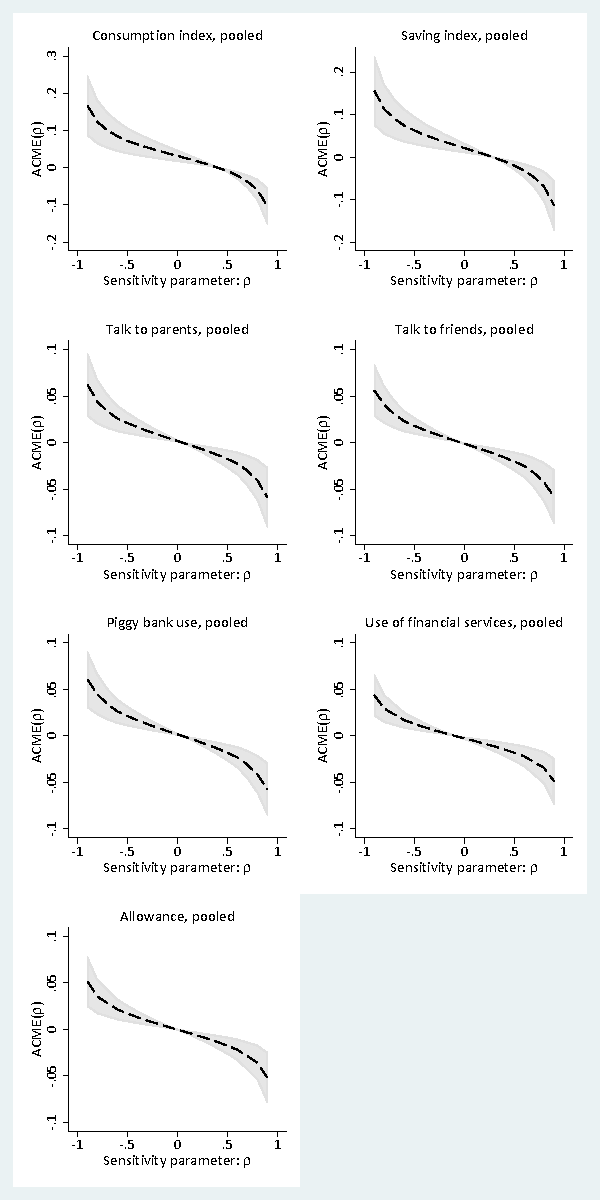
\includegraphics{FigureOA1.pdf}
        \label{fig:te_pooled}

        \raggedright

     {\footnotesize \emph{Note:} Each panel reports the estimated ACME (dashed line) and its 95\% confidence interval (shaded area) as a function of the sensitivity parameter $\rho$, the correlation between the residuals of the mediator and outcome equations (\autoref{eq:oa_med} and \autoref{eq:oa_out}); sequential ignorability implies $\rho = 0$. The consumption and saving indices are standardized attitude indices; the remaining dependent variables are equal to 1 if students talk to parents or friends about financial subjects, if they use a piggy bank, financial services, or receive an allowance from their parents, and 0 otherwise. Sensitivity analysis run with the command \textit{medsens} in \textit{Stata}; standard errors are estimated with bootstrap with 1,000 repetitions. ACME: Average Causal Mediation Effect. }

     {\footnotesize \emph{Source:} Authors' estimates based on the pilot questionnaires applied by CAEd to students at the end of the 2015 school year. }

\end{figure}

\begin{figure} [h!]
		\caption{Sensitivity analysis: average causal mediation effect versus $\rho$, elementary education}
		\centering
		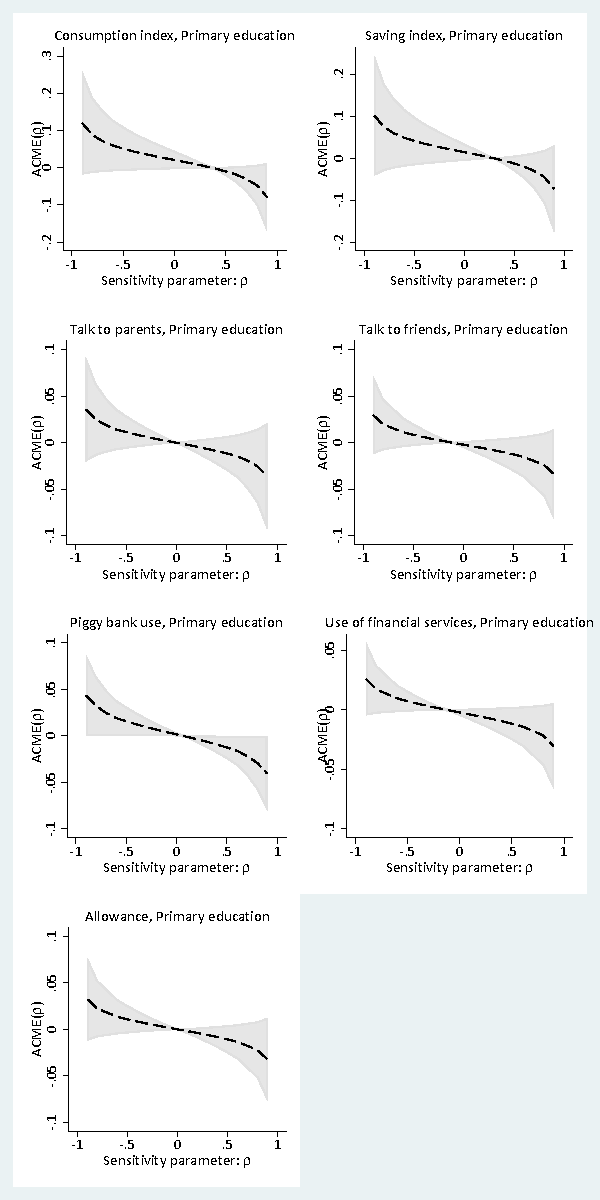
\includegraphics{FigureOA2.pdf}
        \label{fig:te_elementary}

     \raggedright

     {\footnotesize \emph{Note:} See the note to \autoref{fig:te_pooled}. The sample is restricted to elementary school students (fifth grade). }

     {\footnotesize \emph{Source:} Authors' estimates based on the pilot questionnaires applied by CAEd to students at the end of the 2015 school year. }
\end{figure}

\begin{figure} [h!]
		\caption{Sensitivity analysis: average causal mediation effect versus $\rho$, middle school}
		\centering
		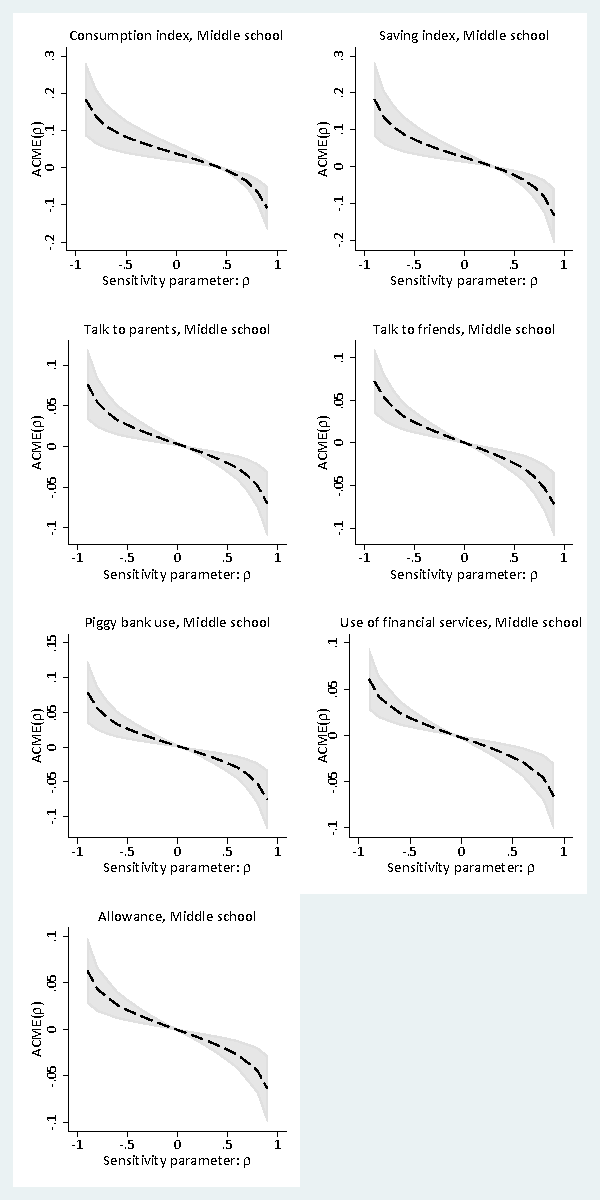
\includegraphics{FigureOA3.pdf}
        \label{fig:te_midle}

                \raggedright

     {\footnotesize \emph{Note:} See the note to \autoref{fig:te_pooled}. The sample is restricted to middle school students (seventh and ninth grades). }

     {\footnotesize \emph{Source:} Authors' estimates based on the pilot questionnaires applied by CAEd to students at the end of the 2015 school year. }
\end{figure}


\newpage
\restoregeometry

\subsection{Robustness to the level of clustering} \label{sec:oa_cluster}

In the paper, standard errors are clustered at the school level, the randomization unit. Because the program was delivered by teachers to their own classes, shocks may also be correlated within classes, so we verify that the inference does not depend on this choice. \autoref{tab:oa_cluster} re-estimates the ITT effects of Table 3 of the paper with the same specification, sample, and outcomes, changing only the level of clustering from the school to the class. The two inference procedures are recomputed accordingly: the Romano--Wolf stepdown p-values treat the same 19 regressions as a single family, with the bootstrap resampling class clusters within randomization strata, and the randomization-inference p-values still reassign the treatment across schools within strata, the actual randomization design, with the test statistic computed under class clustering. The point estimates are identical by construction. The class-clustered standard errors are slightly smaller than the school-clustered ones, and the pattern of statistical significance is the same in 18 of the 19 cells; the only change is financial proficiency among middle school students, whose Romano--Wolf p-value falls from 0.015 to 0.007. The conclusions of the paper are therefore unchanged.

\begin{table}[h!]
\centering
\begin{threeparttable}
\fontsize{9}{10}\selectfont
\caption{ITT estimates for financial proficiency and savings and consumption index, class-clustered standard errors}\label{tab:oa_cluster}
\begin{tabular*}{\textwidth}{@{\extracolsep{\fill}}l*{7}{c}}
\toprule
 & (1) & (2) & (3) & (4) & (5) & (6) & (7) \\
 & Pooled & Elementary & Middle school & Third grade & Fifth grade & Seventh grade & Ninth grade \\
\midrule
\tablefragment{../Datawork/Output/Tables/TableOA1.tex}
\bottomrule
\end{tabular*}
\begin{tablenotes}
\fontsize{9}{9}\selectfont
\item \textit{Notes}: Standard errors clustered at the class level in parentheses; the corresponding school-clustered estimates are reported in Table 3 of the paper, and the point estimates are identical. RW denotes Romano-Wolf stepdown p-values (1{,}000 bootstrap replications resampling class clusters within randomization strata), adjusting for the joint testing of the 19 regressions reported in this table (every outcome in every subsample) as a single family, and RI denotes randomization inference (1{,}000 repetitions reassigning the treatment across schools within strata, the actual randomization design, with the test statistic computed under class clustering); both are reported below the standard error. Stars denote significance levels based on the Romano-Wolf adjusted p-value: * 10\%, ** 5\%, *** 1\%. All three indices are normalized to standard-deviation units. The questionnaire on hypothetical consumption and saving attitudes was not administered to third graders; for these two outcomes, column (4) is therefore empty and column (2) reports the same estimates as column (5), the fifth grade.
\item \textit{Source}: Authors' estimates based on the pilot questionnaires applied by CAEd to students at the end of the 2015 school year.
\end{tablenotes}
\end{threeparttable}
\end{table}

\bibliography{referencesp1}

\end{document}
